\section{Cloud Computing}

Im folgenden Unterkapitel werden die Grundlagen und eine Definition des Cloud Computing erarbeitet um den Kontext dieser Arbeit herleiten zu können.
Hierbei wird vorallem auf die Definition des Cloud Computing nach dem NIST und einiger Grundlagen nach Reinheimer2018 eingegangen.

\subsection{Was ist Cloud Computing}

Cloud Computing ist ein Modell der Zurverfügungstellung eines universell erreichbaren,
günstigen Netzwerkzugangs zu einer Ansammlung konfigurierbarer Computing Ressourcen
(z.B. Netzwerke, Server, Speicher, Anwendungen und Services), die mit minimalem Managementaufwand schnell freigegeben und bereitgestellt werden können
\cite[Vgl.][S. 2]{Mell2011}.

\begin{wrapfigure}{r}{0.45\textwidth}
\centering
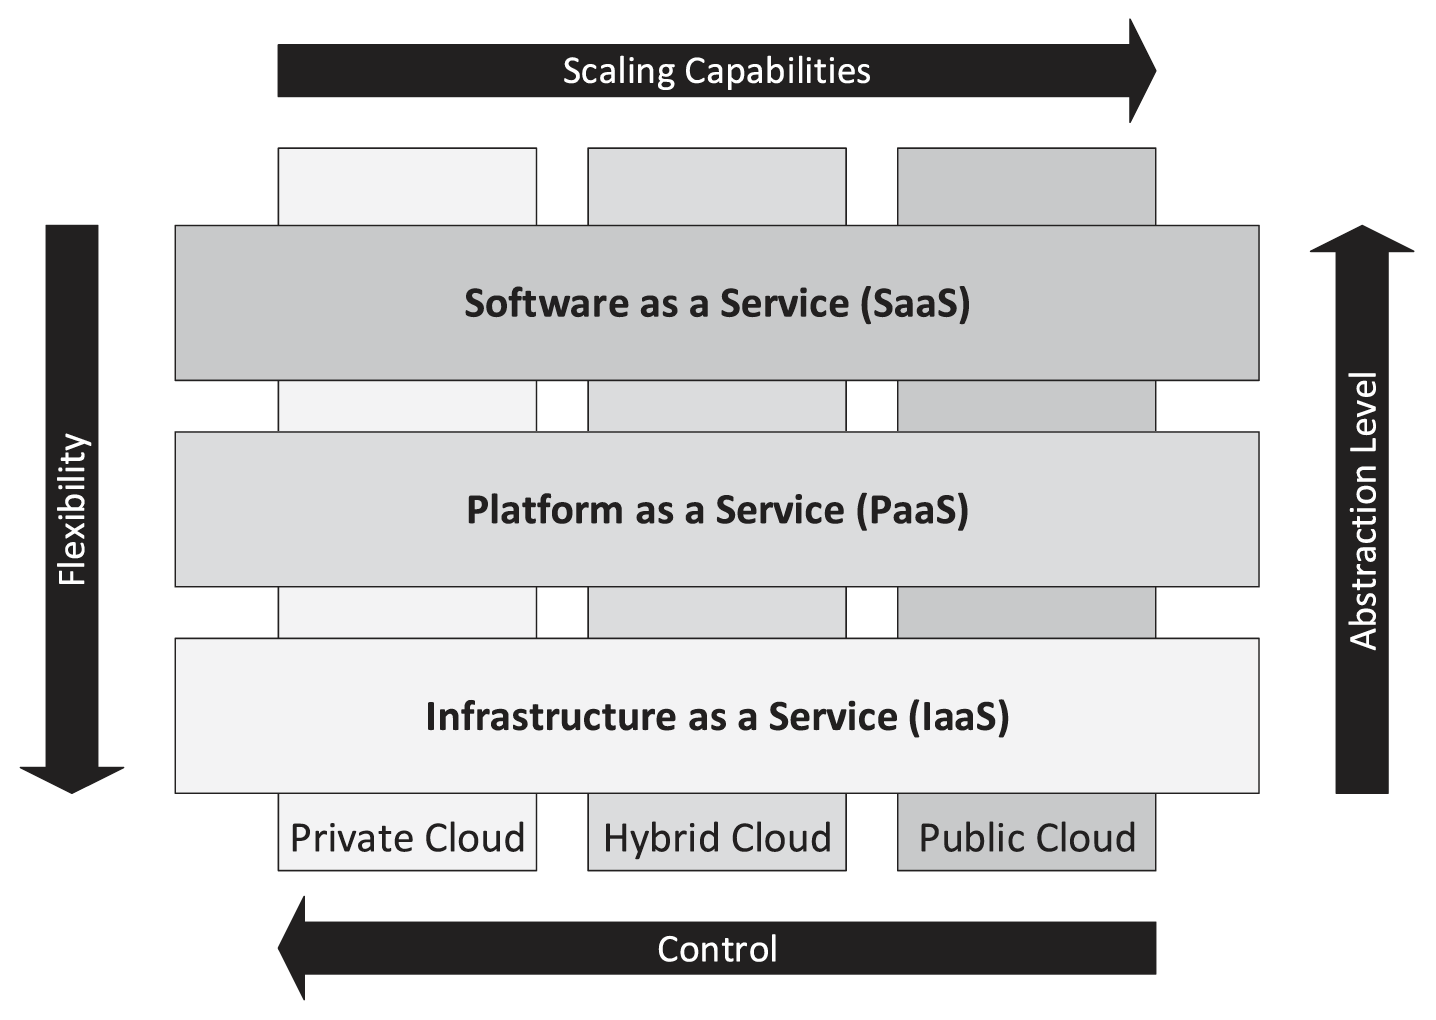
\includegraphics[height=0.35\textwidth]{xaas_maenhaut.png}
\caption{Eine Übersicht der Cloud Service Modelle \cite{Maenhaut2016}}
\end{wrapfigure}

Nach Hentschel und Leyh (2018) kann man Cloud Services grundsätzlich in drei Abstraktionsebenen einteilen. Diese sind \acf{SaaS},
\acf{PaaS} und \acf{IaaS}, welche auch zu \acf{XaaS} zusammengefasst werden
\cite[Vgl.][S. 9]{Reinheimer2018}.

Die unterste der drei genannten Abstraktionsschichten ist die \acf{IaaS}, welche die Basisinfrastruktur, wie zum Beispiel Netzwerk, Server oder Speicher,
bereitstellt. Diese Infrastruktur kann sowohl physisch als auch virtuell zur Verfügung gestellt werden \cite[Vgl.][S. 9f]{Reinheimer2018}.
Die darüberliegende Schicht ist die \acf{PaaS}, welche auf der Infrastruktur zusätzlich noch eine Basis zur Anwendungsentwicklung bietet, indem zum Beispiel
bereits ein Betriebssystem und eine Datenbank installiert sind oder eine andere Programmierumgebung verwendet werden kann \cite[Vgl.][S. 10]{Reinheimer2018}.
Die darüberliegende Schicht ist die \acf{SaaS}, welche standardisierte Anwendungen zur Verfügung stellt und sich somit direkt an den Endnutzer richtet
\cite[Vgl.][S. 11]{Reinheimer2018}.

\subsection{Entwicklung des Cloud Computing}

Die Entwicklung des Cloud Computing und dessen Vorgängerkonzepte is bis in die 90er Jahre zurückzuführen.
Ein von Hentschel und Leyh (2018) hervorgehobender Vorgänger ist das sogrnannte Grid Computing.
Damit war bereits eine dezentrale Ressourcenkontrolle mir standardisierten Protokollen und
Schnittstellen realisiert. Das Cloud Computing bietet vergleichbare Eigenschaften, jedoch rückt der
Fokus hier auf wirtschaftliche Kriterien und die Zenralisierung von Ressourcen zum Beispiel in
Rechenzentren \cite[Vgl.][S. 5f]{Reinheimer2018}.

Nach Srivastava et al. (2018) war Salesforces eines der ersten Unternehmen, welches 1999 Anwendungen über eine Webseite bereitgestellt hat,
gefolgt von den \acf{AWS} in 2002, welche Speicher und Rechenleistung als Services bereitstellten \cite[Vgl.][S. 17f]{Srivastava2018}.

Durch die Entwicklungen im Cloud Computing haben sich drei Basiskomponenten entwickelt \cite[Vgl.][S. 18]{Srivastava2018}:
\begin{itemize}
\item \textbf{Client Computer: }Über die Engeräte kann der Nutzer mit den Services der Cloud interagieren.
\item \textbf{Verteilte Server: }Die Server können verteilt über viele Orte stehen, funktionieren jedoch, wie ein zusammenhängendes System.
\item \textbf{Rechenzentren: }Die Rechenzentren bilden den Knotenpunkt für alle Server und beinhalten selbst weitere Server.
\end{itemize}

\pagebreak

\subsection{Herausforderungen -> Migration von Legacy Anwendungen}

Aus der vorangehend erläuterten Entwicklung des Cloud Computing ergeben sich verschiedene Herausforderungen.
Darunter fällt unter anderem die Migration von Legacy Anwendungen zu Cloud Anwendungen, welche gegeben durch die verschiedenen Service Level
auf unterschiedlichen Wegen realisiert werden kann.